\documentclass{standalone}

\usepackage{pgfplots}

\pgfplotsset{
  compat=1.17,
  samples=100,
  no markers,
  every axis/.append style={
    xlabel={$\bar{L}$},
    grid=both,
    label style={font=\Large},
    tick label style={font=\large}
  },
  every axis plot/.append style={
    blue,
    thick
  }
}

\begin{document}

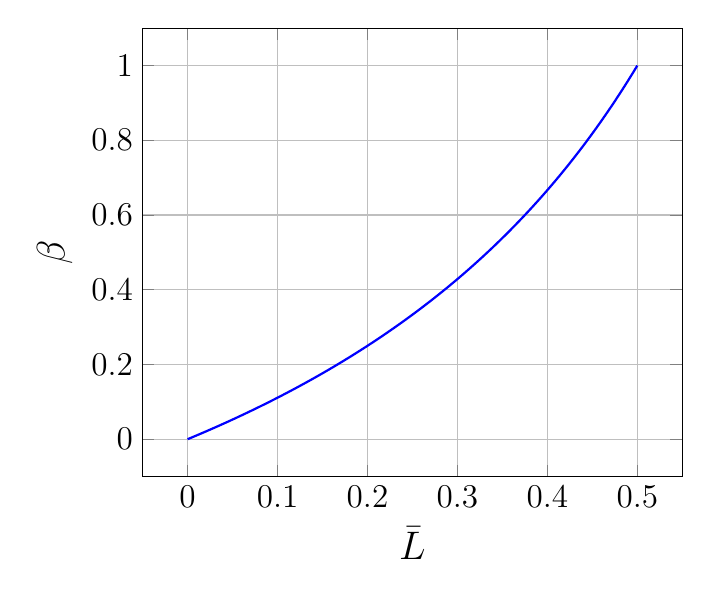
\begin{tikzpicture}
  \begin{axis}[
    ylabel={$\beta$}
  ]
    \addplot[domain=0:0.5] {x / (1 - x)};
  \end{axis}
\end{tikzpicture}
\quad
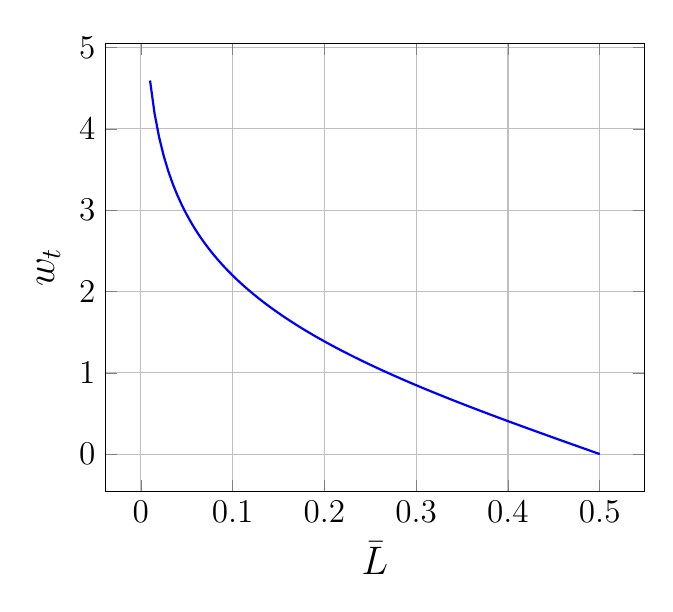
\begin{tikzpicture}
  \begin{axis}[
    ylabel={$w_t$}
  ]
    \addplot[domain=0.01:0.5] {-ln(x / (1 - x))};
  \end{axis}
\end{tikzpicture}

\end{document}
